\documentclass[conference]{IEEEtran}
\IEEEoverridecommandlockouts
\usepackage{cite}
\usepackage{amsmath,amssymb,amsfonts}
\usepackage{graphicx}
\usepackage{textcomp}
\usepackage{xcolor}
\usepackage{booktabs}
\usepackage{url}
\graphicspath{{figures/}}

\begin{document}

\title{Do Situational Attributes Transfer Across Cities? Predicting Crime Near ATMs from New York City to Chicago and Los Angeles}

% TODO: replace the placeholders below with the real author names, departments and contact details.
\author{\IEEEauthorblockN{1\textsuperscript{st} Author Name}
\IEEEauthorblockA{\textit{Department} \\
\textit{Organization}\\
City, Country \\
email address or ORCID}
\and
\IEEEauthorblockN{2\textsuperscript{nd} Author Name}
\IEEEauthorblockA{\textit{Department} \\
\textit{Organization}\\
City, Country \\
email address or ORCID}
\and
\IEEEauthorblockN{3\textsuperscript{rd} Author Name}
\IEEEauthorblockA{\textit{Department} \\
\textit{Organization}\\
City, Country \\
email address or ORCID}
}

\maketitle

\begin{abstract}
Banks and police departments want to know which automated teller machine (ATM) sites are most exposed to crime, and
cities without labelled history would benefit from models trained elsewhere. We test whether situational attributes
of an ATM site improve out-of-sample prediction of nearby robbery and burglary beyond the site's crime history, and
whether such a model transfers from New York City to Chicago and Los Angeles. The attributes are street-light
outages, bars, liquor stores, late-night and all-night venues, rail stations, police stations, highways, branch
opening hours and ATM and branch age. Using 1,790 ATM site-years from public police, OpenStreetMap, 311 and
deposit data, we train logistic regression and LightGBM on 2024 and evaluate on 2025. We use spatially purged folds,
a block bootstrap and a protocol committed to version control before outcomes were linked. A model trained in New
York City and applied to Chicago reached an average precision of 0.731 and ROC-AUC of 0.773 with the attributes,
compared with 0.764 and 0.793 for crime history alone. Adding a random ten percent of Chicago's previous year did not
help in any of twenty draws. Rail-station distance and late-night venues received over a quarter of LightGBM's split
gain, yet removing them barely changed Chicago accuracy. Past crime alone ranked the riskiest tenth of ATMs with
near-perfect precision in all three cities. The attributes showed a promising signal only for incidents recorded at
the ATM itself, which we report as a hypothesis for future validation.
\end{abstract}

\begin{IEEEkeywords}
crime prediction, ATM security, transfer learning, LightGBM, spatial cross-validation, feature importance, negative results
\end{IEEEkeywords}

\section{Introduction}
Crime near automated teller machines (ATMs) combines a predictable cash source with people who are distracted while
withdrawing money, which makes ATM sites a classic problem for situational crime prevention~\cite{scott2001,clarke1999}.
Routine activity theory explains crime as the convergence of a motivated offender, a suitable target and the absence
of a capable guardian~\cite{cohen1979}. This suggests that properties of the site itself (lighting, nearby alcohol
outlets, night-time activity, distance to police) should carry risk information. Crime-and-place research adds that
crime concentrates in a small number of places and persists there from year to year~\cite{weisburd2015,johnson2004}.

These two views lead to a practical question. Most cities do not have a long labelled history of crime at each ATM.
If situational attributes capture the mechanism behind ATM crime, a model learned in a data-rich city should
transfer to other cities. If, instead, the information is largely carried by local crime history, the attributes
will add little and may not transfer at all.

We study this question for New York City (NYC), Chicago and Los Angeles (LA), training on NYC and predicting
Chicago and LA. Our contributions are:
\begin{itemize}
\item A reproducible open-data pipeline that links 962 mapped ATM and bank objects to police incidents, 311
street-light requests, OpenStreetMap points of interest and FDIC branch deposits, with all attributes measured
before the outcome year.
\item A pre-specified, spatially purged evaluation of logistic regression and LightGBM, including a few-shot setting
in which ten percent of the target city's previous year is added to training.
\item Evidence that the attributes do not improve transfer beyond crime history, and that high feature importance
did not translate into predictive value in the target city.
\item A secondary signal for ATM-premise incidents, reported with its uncertainty as a hypothesis rather than a finding.
\end{itemize}

\section{Related Work}
\textit{Crime concentration and history.} Crime is concentrated at a small share of street segments and is stable
over time~\cite{weisburd2015}. Recent victimization predicts near-future risk nearby~\cite{johnson2004}, and
self-exciting point processes formalize this persistence~\cite{mohler2011}.

\textit{Environmental risk factors.} Crime generators and attractors such as bars and transit hubs raise local risk
\cite{brantingham1995}. Risk terrain modeling combines such layers into a risk surface~\cite{caplan2011}, and machine
learning variants have been proposed~\cite{wheeler2021}. ATM-specific guidance emphasizes lighting, visibility and
siting~\cite{scott2001}.

\textit{Evaluation and transfer.} Spatially autocorrelated data inflate accuracy under random cross-validation, so
blocked or purged schemes are recommended~\cite{roberts2017}. For rare outcomes, precision-recall summaries are more
informative than ROC curves~\cite{saito2015}. Transfer learning studies when knowledge from a source domain helps a
target domain~\cite{pan2010}. Gradient-boosted trees remain strong on tabular data~\cite{ke2017,grinsztajn2022}, and
SHAP values attribute their predictions to features~\cite{lundberg2017}. However, importance measures can be biased
and need not reflect out-of-sample value~\cite{strobl2007}.

\section{Data}
\subsection{ATM Sites and Outcomes}
ATM and bank objects (\texttt{amenity=atm}, or \texttt{amenity=bank} with \texttt{atm=yes}) were reconstructed from
108 monthly OpenStreetMap snapshots, February 2023 to January 2026, retrieved through the ohsome
framework~\cite{raifer2019}. A site-year is an object present for the full calendar year. We use a conservative core
that keeps point objects with at most 10 m of coordinate drift, no other object within 10 m and an untruncated 500 m
buffer inside the city. This yields 1,790 site-years from 962 distinct objects (Table~\ref{tab:cohort}). OSM
positions are mapped locations rather than verified machine positions~\cite{haklay2010}.

Incidents come from the NYPD complaint data, the Chicago Police Department crime data and the LAPD crime and NIBRS
files~\cite{nycopen,chiopen,laopen}. Robbery and structural burglary were harmonized across cities; 9,192
vehicle-burglary cases (NYC truck burglary and Chicago theft from motor vehicle) were excluded from outcomes and
predictors alike. The primary outcome is any robbery or burglary within 50 m of the released ATM coordinates during
the outcome year. A secondary outcome is any incident whose police premise code is ATM within 100 m (NYC and Chicago;
LA's 2025 coordinates are rounded to about 1 km). Released crime coordinates are themselves approximate, especially
Chicago's block-level locations, so the outcome measures proximity rather than confirmed attacks on a machine.

\begin{table}[t]
\caption{Cohort: site-years and sites with robbery or burglary within 50\,m}
\label{tab:cohort}
\centering
\begin{tabular}{lcccc}
\toprule
& \multicolumn{2}{c}{2024 (training)} & \multicolumn{2}{c}{2025 (test)} \\
City & Sites & With crime & Sites & With crime \\
\midrule
New York City & 557 & 350 (63\%) & 611 & 345 (56\%) \\
Chicago & 190 & 111 (58\%) & 212 & 87 (41\%) \\
Los Angeles & 108 & 37 (34\%) & 112 & 37 (33\%) \\
\midrule
Total & 855 & 498 & 935 & 469 \\
\bottomrule
\end{tabular}
\end{table}

\subsection{Crime-History Baseline}
The baseline uses two predictors measured in the year before the outcome: the log count of incidents within 50 m of
the site and the log count at 200--500 m. These capture local persistence and the surrounding level of crime.

\subsection{Situational Attributes}
Table~\ref{tab:attr} lists the 15 attributes. OSM layers come from the snapshot of 15 December before the outcome
year; 311 requests cover the preceding calendar year. Counts and distances (capped at 5 km) are log-transformed.
Some requested attributes could not be measured. Cash-replenishment schedules are not public. True installation
dates are unavailable, so we use the time since the object was first mapped. Direct night-time pedestrian counts
are not openly available on a comparable basis, so we use night-time venues and rail access as proxies. OSM street
lamps were excluded because far fewer lamps are mapped than exist, so a count would mostly measure mapping effort.
A licence-based alcohol-outlet variant was withdrawn before outcome linkage: the New York licence register's issue
dates cannot reconstruct which licences were active in 2023 and 2024.

\begin{table}[t]
\caption{Situational attributes (all measured before the outcome year)}
\label{tab:attr}
\centering
\begin{tabular}{p{3.6cm}p{3.9cm}}
\toprule
Attribute & Source and definition \\
\midrule
Street-light outages & 311 failure requests within 100 m \\
Bars; liquor stores & OSM count within 250 m and nearest distance (4 features) \\
Late-night venues & OSM fast food, cinema, theatre, casino, fuel, convenience within 250 m \\
All-night venues & OSM objects open 24/7 within 250 m \\
Rail or subway station & distance to nearest (OSM) \\
Police station & distance to nearest (OSM) \\
Highway & distance to nearest motorway or trunk (OSM) \\
Branch hours & hours listed; open weekends; open late \\
ATM age & years since first mapped (OSM history) \\
Branch age & years since the co-located FDIC branch opened~\cite{fdic} \\
\bottomrule
\end{tabular}
\end{table}

Coverage differs by city. Opening hours are listed for 50--56\% of NYC sites, but only 7--22\% of Chicago sites and
17--20\% of LA sites. OSM records far more liquor stores near NYC sites than near Chicago or LA sites, partly
reflecting mapping density. The 311 data contain 24,000--26,000 qualifying street-light requests per year in NYC,
about 46,000 in Chicago and 32,000--46,000 in LA, so request volumes also reflect local reporting practice.

\section{Methods}
\subsection{Models}
The logistic baseline (M0) is
\begin{equation}
\Pr(y_i=1)=\sigma\left(\beta_0+\beta_1 x_{i}^{(50)}+\beta_2 x_{i}^{(200\text{--}500)}\right),\label{eq:m0}
\end{equation}
where $\sigma$ is the logistic function and $x_i^{(50)}$ and $x_i^{(200\text{--}500)}$ are the log prior-year counts.
M9 adds the 15 attributes. Logistic models use median imputation, standardization and an L2 penalty with
$C\in\{0.01,0.1,1,10\}$~\cite{pedregosa2011}. LightGBM~\cite{ke2017} uses a learning rate of 0.03, row and column
subsampling of 0.8 and L2 regularization of 1. The grid covers 4, 8 or 16 leaves, a minimum of 20 or 40 samples per
leaf and 100 or 300 trees. Missing values are handled natively and training is deterministic. All hyperparameters
are chosen by three-fold inner cross-validation on 2\,km spatial blocks within the training data, with purging.

\subsection{Designs}
All designs train on 2024 outcomes and test on 2025 outcomes.
\textit{Transfer} trains on NYC only and tests on Chicago (primary) and LA.
\textit{Few-shot transfer} adds a random 10\% of Chicago's 2024 site-years (19 rows). The Chicago test set is split
into five folds of 2\,km blocks, and for each fold the sample is drawn only from Chicago 2024 sites at least 1,500 m
from, and sharing no census geography with, that fold's test sites. This is repeated over 20 random seeds.
\textit{Full adaptation} uses all eligible Chicago 2024 rows under the same purge.
\textit{Pooled within-city} trains on all three cities with five purged spatial folds.

\subsection{Metrics, Uncertainty and Pre-registration}
The primary metric is average precision (AP),
\begin{equation}
\mathrm{AP}=\sum_{k}\left(R_k-R_{k-1}\right)P_k,\label{eq:ap}
\end{equation}
where $P_k$ and $R_k$ are precision and recall at the $k$-th threshold~\cite{saito2015}. We also report ROC-AUC and
the Brier score. Paired differences use 2,000 bootstrap resamples of 2\,km test blocks within each city~\cite{efron1993}.
The protocol, including the attributes, designs, learners and success rule, was committed to version control before
any attribute was joined to an outcome. Success required an AP gain of at least 0.01 for M9 over logistic M0 on
NYC-to-Chicago, a Bonferroni-adjusted lower bound above zero for the two primary contrasts, and no worse Brier
score. The few-shot design and the weightage analysis were added afterwards and are exploratory. Roughly 45
secondary contrasts are reported without multiplicity correction.

\subsection{Weightage}
For LightGBM we report each feature's share of total split gain, its share of mean absolute SHAP
value~\cite{lundberg2017}, and the drop in Chicago AP when the feature is permuted.

\section{Results}
\subsection{Transfer from NYC to Chicago}
Table~\ref{tab:chicago} and Fig.~\ref{fig:perf} show that crime history alone gave the best Chicago predictions. With
the attributes, LightGBM reached AP 0.731 and ROC-AUC 0.773, against 0.764 and 0.793 for logistic M0. The AP
difference was $-0.033$ (Bonferroni interval $-0.084$ to $+0.026$). Logistic M9 fell further, to AP 0.712. The
primary success rule was not met. The attribute models had lower Brier scores (0.201 against 0.213). This mostly
reflects a shift in the average predicted probability towards Chicago's lower crime rate, not better ranking of sites.

\begin{table}[t]
\caption{Chicago 2025 performance (212 sites, 87 with crime)}
\label{tab:chicago}
\centering
\setlength{\tabcolsep}{4pt}
\begin{tabular}{lcccccc}
\toprule
& \multicolumn{2}{c}{NYC only} & \multicolumn{2}{c}{NYC + 10\%} & \multicolumn{2}{c}{NYC + all} \\
Model & AP & AUC & AP & AUC & AP & AUC \\
\midrule
Logistic M0 (baseline) & \textbf{0.764} & \textbf{0.793} & \textbf{0.764} & \textbf{0.794} & \textbf{0.768} & \textbf{0.797} \\
LightGBM M0 & 0.742 & 0.771 & 0.735 & 0.766 & 0.737 & 0.776 \\
LightGBM M9 & 0.731 & 0.773 & 0.722 & 0.763 & 0.733 & 0.779 \\
Logistic M9 & 0.712 & 0.765 & -- & -- & 0.751 & 0.781 \\
\bottomrule
\multicolumn{7}{p{8.2cm}}{\footnotesize NYC + 10\%: mean over 20 random draws of 19 Chicago 2024 site-years.
Random ranking gives AP 0.41 and AUC 0.50.}
\end{tabular}
\end{table}

\begin{figure*}[t]
\centerline{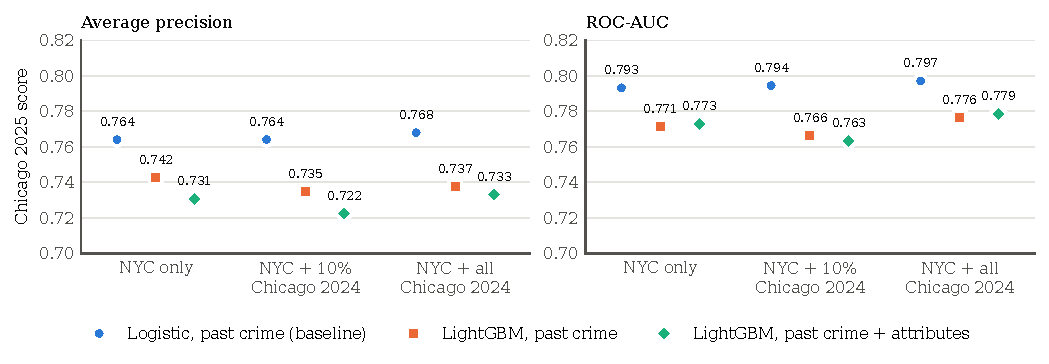
\includegraphics[width=0.85\textwidth]{chicago_performance.pdf}}
\caption{Chicago 2025 average precision and ROC-AUC by training data. Crime history with logistic regression
(circles) scores highest in every setting; adding the attributes to LightGBM (diamonds) does not close the gap.}
\label{fig:perf}
\end{figure*}

\subsection{Adding Chicago Data}
Adding a random 10\% of Chicago's 2024 site-years lowered LightGBM M9 to a mean AP of 0.722 (range 0.679--0.740) and
an AUC of 0.763. It beat logistic M0 in none of the 20 draws; the draw-averaged difference was $-0.042$ (95\%
interval $-0.089$ to $+0.013$). Using all eligible Chicago rows did not change the ordering
(Table~\ref{tab:chicago}). Small target samples were not enough to recalibrate what the attributes mean in Chicago.

\subsection{Los Angeles and Pooled Within-City Prediction}
On LA (112 sites, 37 with crime), logistic M9 lost 0.101 AP against M0 (95\% interval $-0.200$ to $-0.029$).
LightGBM M9 matched M0 on AP (0.777 against 0.781) with a slightly higher AUC (0.852 against 0.840). In the pooled
three-city design, logistic M9 and M0 were equal on AP (0.805 against 0.804), while M9 raised AUC from 0.794 to
0.808. The attributes helped slightly in NYC (AP 0.820 to 0.831) and hurt in Chicago (0.765 to 0.738) and LA
(0.785 to 0.713). This pattern is consistent with relationships learned mostly from NYC, the largest city.

\subsection{Attribute Weightage}
Fig.~\ref{fig:weight} shows LightGBM's split-gain shares. The two crime-history features took 41.6\% of the gain
when training on NYC alone and 39.7\% with the Chicago sample. Rail-station distance (13.3\%), late-night venues
(11.8\%), ATM age (7.6\%), all-night venues (6.8\%) and liquor-store distance (6.6\%) followed. Street-light outages,
bar counts, liquor-store counts and branch hours each took under 1\%. Higher values of past crime, late-night venues
and ATM age raised predicted risk; proximity to rail stations, liquor stores and highways also raised it.

Importance did not translate into value in Chicago. Permuting prior local crime lowered Chicago AP by 0.238.
Permuting any attribute changed it by at most 0.019, and permuting late-night venues improved it by 0.017. SHAP
shares on the Chicago test set ranked the features similarly to the NYC gain shares. The model used the same
features in both cities, but their relationship with crime differed.

\begin{figure}[t]
\centerline{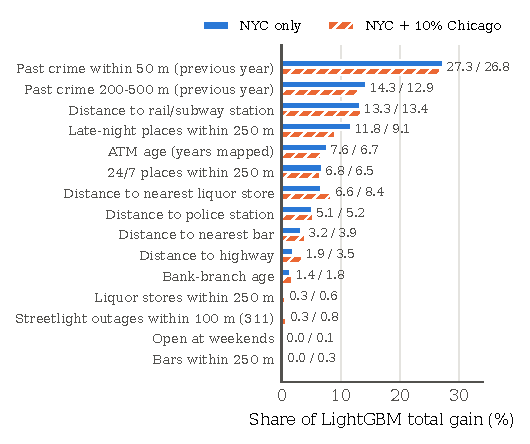
\includegraphics[width=\columnwidth]{weightage.pdf}}
\caption{LightGBM weightage (share of total split gain, \%) for NYC-only training and NYC plus 10\% of Chicago 2024
(mean of 100 models). Labels give both values. Two branch-hours features with zero gain in both settings are omitted.}
\label{fig:weight}
\end{figure}

\subsection{ATM-Premise Incidents}
For the secondary outcome in the pooled design (823 NYC and Chicago test sites, 137 with an ATM-premise incident),
the attributes raised logistic AP from 0.188 to 0.248 (95\% interval for the gain $+0.009$ to $+0.100$) and AUC
from 0.577 to 0.643. Adding branch deposits and branch presence raised AP to 0.275 and AUC to 0.694. An earlier
stage of this project found that deposits at a co-located branch predict ATM-premise incidents, with rates rising
from 11.9\% to 35.0\% across deposit quintiles, while general robbery and burglary rates stayed between 56\% and
65\% across the same quintiles. The
gain is concentrated in NYC (AP 0.212 to 0.277) and does not transfer from NYC to Chicago (AP change $-0.016$). Given
the number of secondary comparisons, we treat it as a hypothesis.

\subsection{Practical Ranking}
Although the attributes did not help, the transferred crime-history model ranked sites well (Table~\ref{tab:rank}).
All 21 Chicago ATMs and all 11 LA ATMs in its riskiest tenth had a robbery or burglary within 50 m in 2025, against
city-wide rates of 41\% and 33\%. LightGBM with attributes reached 86\% and 91\%.

\begin{table}[t]
\caption{Share of the riskiest 10\% of ATMs with crime in 2025}
\label{tab:rank}
\centering
\setlength{\tabcolsep}{3.5pt}
\begin{tabular}{lcccc}
\toprule
& Base & Top 10\%, & Top 10\%, & Bottom 50\%, \\
City & rate & logistic M0 & LightGBM M9 & logistic M0 \\
\midrule
Chicago$^{a}$ & 41\% & 100\% (21/21) & 86\% & 21\% \\
Los Angeles$^{a}$ & 33\% & 100\% (11/11) & 91\% & 11\% \\
New York City$^{b}$ & 56\% & 97\% (59/61) & 89\% & 37\% \\
\bottomrule
\multicolumn{5}{l}{\footnotesize $^{a}$Trained on NYC only. $^{b}$Pooled design, spatially purged folds.}
\end{tabular}
\end{table}

\section{Discussion}
\textit{Why the attributes did not transfer.} First, crime history already summarizes much of what the attributes
measure: a site near a busy station or late-night strip has usually had crime before. Second, the meaning of an
attribute is city-specific. Rail stations, late-night venues and liquor stores sit in very different urban contexts
in NYC, Chicago and LA, and the training base rates differ (63\% in NYC against 41\% in Chicago). Third, several
measures are proxies with uneven coverage. OSM completeness varies~\cite{haklay2010}, 311 volumes reflect reporting
habits, and opening hours are sparsely tagged outside NYC.

\textit{Importance is not evidence of value.} LightGBM assigned over half of its gain to attributes, yet none improved
Chicago accuracy. Feature importance describes what a fitted model uses on its training distribution~\cite{strobl2007}.
A claim that an attribute matters for prediction needs an out-of-sample comparison against a strong baseline.

\textit{Implications.} For a city with crime records but no ATM-specific model, ranking sites by recent nearby crime is
a simple and accurate first step. Situational features may still matter for ATM-premise incidents, where target
supply (cash volume and footfall) is a plausible mechanism. That is the outcome to pursue with independently
validated site measurements.

\textit{Limitations.} The 2024 and 2025 outcomes were examined in earlier stages of this project, so the evaluation
is retrospective even though the Restart~9 protocol was fixed beforehand. Test samples are modest (212 Chicago and
112 LA sites), and intervals are wide. Locations of ATMs and incidents are approximate, and the cohort keeps only
sites mapped for a full year. Premise coding is an officer's judgment. The few-shot design and weightage analysis
were added after the primary result was known.

\section{Conclusion}
We asked whether lighting, alcohol outlets, night-time activity, police and highway access, branch hours and ATM age
improve prediction of crime near ATMs beyond crime history, and whether a model trained in New York City transfers
to Chicago and Los Angeles. Under a pre-specified, spatially purged evaluation, they did not. Neither logistic
regression nor LightGBM with the attributes beat a two-variable crime-history baseline in Chicago, and a small
sample of Chicago data did not change this. Several attributes received high LightGBM importance without improving
target-city accuracy. Future work should validate the ATM-premise signal on an unseen year with a frozen
specification, and should obtain verified ATM locations and direct site observations.

\section*{Data and Code Availability}
All inputs are public: OpenStreetMap (ODbL) via ohsome, NYC, Chicago and LA open-data portals including 311, and the
FDIC Summary of Deposits. Code, the frozen protocol, amendments, raw-file hashes and all predictions are in the
project repository [repository URL].

\begin{thebibliography}{00}
\bibitem{scott2001} M. S. Scott, ``Robbery at automated teller machines,'' Problem-Oriented Guides for Police,
Problem-Specific Guides Series, no. 8, U.S. Department of Justice, Office of Community Oriented Policing Services,
Washington, DC, 2001.
\bibitem{clarke1999} R. V. Clarke, ``Hot products: Understanding, anticipating and reducing demand for stolen goods,''
Police Research Series, Paper 112, Home Office, London, 1999.
\bibitem{cohen1979} L. E. Cohen and M. Felson, ``Social change and crime rate trends: A routine activity approach,''
\textit{Amer. Sociol. Rev.}, vol. 44, no. 4, pp. 588--608, 1979.
\bibitem{weisburd2015} D. Weisburd, ``The law of crime concentration and the criminology of place,''
\textit{Criminology}, vol. 53, no. 2, pp. 133--157, 2015.
\bibitem{johnson2004} S. D. Johnson and K. J. Bowers, ``The burglary as clue to the future: The beginnings of
prospective hot-spotting,'' \textit{Eur. J. Criminol.}, vol. 1, no. 2, pp. 237--255, 2004.
\bibitem{mohler2011} G. O. Mohler, M. B. Short, P. J. Brantingham, F. P. Schoenberg, and G. E. Tita,
``Self-exciting point process modeling of crime,'' \textit{J. Amer. Statist. Assoc.}, vol. 106, no. 493,
pp. 100--108, 2011.
\bibitem{brantingham1995} P. L. Brantingham and P. J. Brantingham, ``Criminality of place: Crime generators and
crime attractors,'' \textit{Eur. J. Crim. Policy Res.}, vol. 3, no. 3, pp. 5--26, 1995.
\bibitem{caplan2011} J. M. Caplan, L. W. Kennedy, and J. Miller, ``Risk terrain modeling: Brokering criminological
theory and GIS methods for crime forecasting,'' \textit{Justice Quart.}, vol. 28, no. 2, pp. 360--381, 2011.
\bibitem{wheeler2021} A. P. Wheeler and W. Steenbeek, ``Mapping the risk terrain for crime using machine learning,''
\textit{J. Quant. Criminol.}, vol. 37, pp. 445--480, 2021.
\bibitem{roberts2017} D. R. Roberts \textit{et al.}, ``Cross-validation strategies for data with temporal, spatial,
hierarchical, or phylogenetic structure,'' \textit{Ecography}, vol. 40, no. 8, pp. 913--929, 2017.
\bibitem{saito2015} T. Saito and M. Rehmsmeier, ``The precision-recall plot is more informative than the ROC plot
when evaluating binary classifiers on imbalanced datasets,'' \textit{PLoS ONE}, vol. 10, no. 3, e0118432, 2015.
\bibitem{pan2010} S. J. Pan and Q. Yang, ``A survey on transfer learning,'' \textit{IEEE Trans. Knowl. Data Eng.},
vol. 22, no. 10, pp. 1345--1359, 2010.
\bibitem{ke2017} G. Ke \textit{et al.}, ``LightGBM: A highly efficient gradient boosting decision tree,'' in
\textit{Proc. Adv. Neural Inf. Process. Syst. (NIPS)}, vol. 30, 2017, pp. 3146--3154.
\bibitem{grinsztajn2022} L. Grinsztajn, E. Oyallon, and G. Varoquaux, ``Why do tree-based models still outperform
deep learning on typical tabular data?'' in \textit{Proc. Adv. Neural Inf. Process. Syst. (NeurIPS), Datasets and
Benchmarks Track}, 2022.
\bibitem{lundberg2017} S. M. Lundberg and S.-I. Lee, ``A unified approach to interpreting model predictions,'' in
\textit{Proc. Adv. Neural Inf. Process. Syst. (NIPS)}, vol. 30, 2017, pp. 4765--4774.
\bibitem{strobl2007} C. Strobl, A.-L. Boulesteix, A. Zeileis, and T. Hothorn, ``Bias in random forest variable
importance measures: Illustrations, sources and a solution,'' \textit{BMC Bioinformatics}, vol. 8, art. 25, 2007.
\bibitem{pedregosa2011} F. Pedregosa \textit{et al.}, ``Scikit-learn: Machine learning in Python,''
\textit{J. Mach. Learn. Res.}, vol. 12, pp. 2825--2830, 2011.
\bibitem{efron1993} B. Efron and R. J. Tibshirani, \textit{An Introduction to the Bootstrap}. New York, NY, USA:
Chapman \& Hall, 1993.
\bibitem{raifer2019} M. Raifer \textit{et al.}, ``OSHDB: A framework for spatio-temporal analysis of OpenStreetMap
history data,'' \textit{Open Geospatial Data, Softw. Stand.}, vol. 4, art. 3, 2019.
\bibitem{haklay2010} M. Haklay, ``How good is volunteered geographical information? A comparative study of
OpenStreetMap and Ordnance Survey datasets,'' \textit{Environ. Plann. B, Plann. Des.}, vol. 37, no. 4,
pp. 682--703, 2010.
\bibitem{nycopen} City of New York, ``NYPD complaint data historic'' and ``311 service requests,'' NYC Open Data.
[Online]. Available: \url{https://opendata.cityofnewyork.us}
\bibitem{chiopen} City of Chicago, ``Crimes---2001 to present'' and ``311 service requests,'' Chicago Data Portal.
[Online]. Available: \url{https://data.cityofchicago.org}
\bibitem{laopen} City of Los Angeles, ``Crime data,'' ``LAPD NIBRS offenses'' and ``MyLA311 service request data,''
Los Angeles Open Data. [Online]. Available: \url{https://data.lacity.org}
\bibitem{fdic} Federal Deposit Insurance Corporation, ``Summary of Deposits.'' [Online]. Available:
\url{https://www.fdic.gov}
\end{thebibliography}

\end{document}
